\documentclass[aspectratio=169,11pt]{beamer}
\usepackage[T1]{fontenc}
\usepackage{lmodern,amsmath,amssymb,mathtools,bm,booktabs,array,graphicx,tikz}
\usetikzlibrary{arrows.meta,positioning,calc,decorations.pathreplacing,patterns}
\definecolor{ink}{HTML}{17344D}\definecolor{accent}{HTML}{087E8B}\definecolor{pale}{HTML}{EDF5F5}\definecolor{gold}{HTML}{AD6B19}
\providecommand{\dd}{\,\mathrm{d}}\providecommand{\R}{\mathbb{R}}
\providecommand{\E}{\mathbb{E}}\providecommand{\Var}{\operatorname{Var}}
\providecommand{\Cov}{\operatorname{Cov}}\providecommand{\diag}{\operatorname{diag}}
\providecommand{\norm}[1]{\left\lVert#1\right\rVert}
\providecommand{\abs}[1]{\left|#1\right|}
\usefonttheme{professionalfonts}
\setbeamercolor{normal text}{fg=black,bg=white}
\setbeamercolor{frametitle}{fg=ink,bg=white}
\setbeamercolor{title}{fg=ink}\setbeamercolor{structure}{fg=accent}
\setbeamercolor{block title}{fg=ink,bg=pale}\setbeamercolor{block body}{fg=black,bg=pale!40}
\setbeamercolor{alerted text}{fg=accent}
\setbeamerfont{frametitle}{size=\Large,series=\bfseries}
\setbeamerfont{title}{size=\LARGE,series=\bfseries}
\setbeamertemplate{navigation symbols}{}
\setbeamersize{text margin left=.7cm,text margin right=.7cm}
\setbeamertemplate{frametitle}{\vspace{.18cm}\insertframetitle\par\vspace{.1cm}{\color{accent}\hrule height .6pt}\vspace{.12cm}}
\newcommand{\notestarget}{notes.pdf}\newcommand{\noteslabel}{Notes}
\setbeamertemplate{footline}{\hspace{.7cm}\color{ink}\scriptsize Scientific Computing in Python / 2027\quad\href{\notestarget}{\noteslabel}\hfill\insertframenumber\,/\,\inserttotalframenumber\hspace{.7cm}\vspace{.18cm}}
\setbeamercovered{invisible}
\hypersetup{pdfauthor={Zan Ahmad},pdftitle={Functions, array axes, and planar trajectories},pdfpagemode=UseNone}
\begin{document}
\begin{frame}[plain]\vfill
{\small\color{accent} Scientific Computing in Python / 2027 \quad Lecture 2}\par\medskip
{\raggedright\hyphenpenalty=10000\exhyphenpenalty=10000\LARGE\bfseries\color{ink} Functions, array axes, and planar trajectories}\par\bigskip
Zan Ahmad\par\smallskip
{\small Proposed 2027; calendar dates pending}\par\vfill\end{frame}
\renewcommand{\notestarget}{notes.pdf\#note-the-axes-of-a-trajectory-array}
\begin{frame}[t,fragile,label=slide-the-axes-of-a-trajectory-array]{The axes of a trajectory array}
\[
p\in\R^{R\times T\times2},\qquad p_{ri0}=x_{ri},\quad p_{ri1}=y_{ri}.
\]
\pause{}
Time is axis 1. Component is axis 2.
\end{frame}
\renewcommand{\notestarget}{notes.pdf\#note-the-axes-of-a-trajectory-array}
\begin{frame}[t,fragile,label=slide-indexing-an-observation]{Indexing an observation}
\begin{verbatim}
p[r, i, :]       # one two-component position
p[r, :, :]       # one full trajectory
p[:, i, :]       # all positions at one time
\end{verbatim}
\pause{}
Each slice retains a different physical question.
\end{frame}
\renewcommand{\notestarget}{notes.pdf\#note-interval-average-velocity}
\begin{frame}[t,fragile,label=slide-interval-average-velocity]{Interval-average velocity}
\[
v_{ric}=\frac{p_{r,i+1,c}-p_{ric}}{t_{i+1}-t_i}.
\]
\pause{}
The result has shape $(R,T-1,2)$.
\end{frame}
\renewcommand{\notestarget}{notes.pdf\#note-interval-average-velocity}
\begin{frame}[t,fragile,label=slide-broadcasting-the-time-increments]{Broadcasting the time increments}
\begin{verbatim}
dp = np.diff(p, axis=1)
dt = np.diff(t)
v = dp / dt[None, :, None]
\end{verbatim}
\pause{}
The two singleton axes repeat the same interval durations across trajectories and coordinate components.
\end{frame}
\renewcommand{\notestarget}{notes.pdf\#note-magnitude-and-threshold-indicators}
\begin{frame}[t,fragile,label=slide-magnitude-and-threshold-indicators]{Magnitude and threshold indicators}
\[
s_{ri}=\sqrt{v_{ri0}^2+v_{ri1}^2},\qquad I_{ri}=\mathbf1_{\{s_{ri}>s_*\}}.
\]
\pause{}
The strict inequality excludes equality.
\end{frame}
\renewcommand{\notestarget}{notes.pdf\#note-a-rotation-matrix}
\begin{frame}[label=slide-trajectory-rotation-figure]{Trajectory rotation}
\centering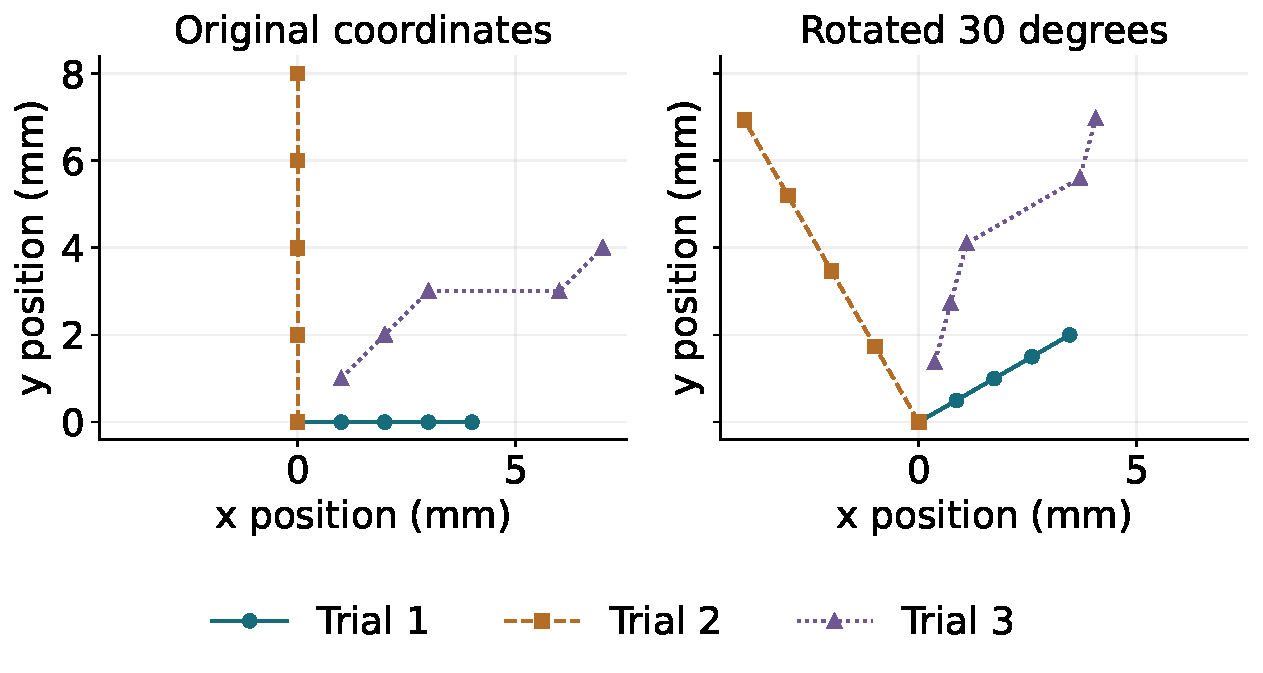
\includegraphics[width=.98\linewidth,height=.69\textheight,keepaspectratio]{trajectory-rotation.pdf}\end{frame}
\renewcommand{\notestarget}{notes.pdf\#note-magnitude-and-threshold-indicators}
\begin{frame}[t,fragile,label=slide-a-threshold-function]{A threshold function}
\begin{verbatim}
def above_threshold(speed, target):
    return speed > target
\end{verbatim}
\pause{}
At $s_*=2$, a speed of $2$ does not qualify and $2.01$ does. Missing and nonfinite inputs require a separate policy.
\end{frame}
\renewcommand{\notestarget}{notes.pdf\#note-a-rotation-matrix}
\begin{frame}[t,fragile,label=slide-a-rotation-matrix]{A rotation matrix}
\[
R(\theta)=\begin{pmatrix}\cos\theta&-\sin\theta\\\sin\theta&\cos\theta\end{pmatrix}.
\]
\pause{}
\[
p'=Rp\quad\text{for columns},\qquad P'=PR^{\mathsf T}\quad\text{for rows}.
\]
\end{frame}
\renewcommand{\notestarget}{notes.pdf\#note-a-rotation-matrix}
\begin{frame}[t,fragile,label=slide-rotation-of-a-basis-vector]{Rotation of a basis vector}
At $\theta=\pi/6$,
\[
R\begin{pmatrix}1\\0\end{pmatrix}=\begin{pmatrix}\sqrt3/2\\1/2\end{pmatrix}.
\]
\pause{}
Its length remains one, while its coordinate components change.
\end{frame}
\renewcommand{\notestarget}{notes.pdf\#note-orthogonality-and-length-preservation}
\begin{frame}[t,fragile,label=slide-orthogonality-and-length-preservation]{Orthogonality and length preservation}
\[
\|R\Delta p\|_2^2=\Delta p^{\mathsf T}R^{\mathsf T}R\Delta p=\|\Delta p\|_2^2.
\]
\pause{}
Thus every interval speed is unchanged.
\end{frame}
\renewcommand{\notestarget}{notes.pdf\#note-interval-average-velocity}
\begin{frame}[label=slide-speed-shape-map-figure]{Speed shape map}
\centering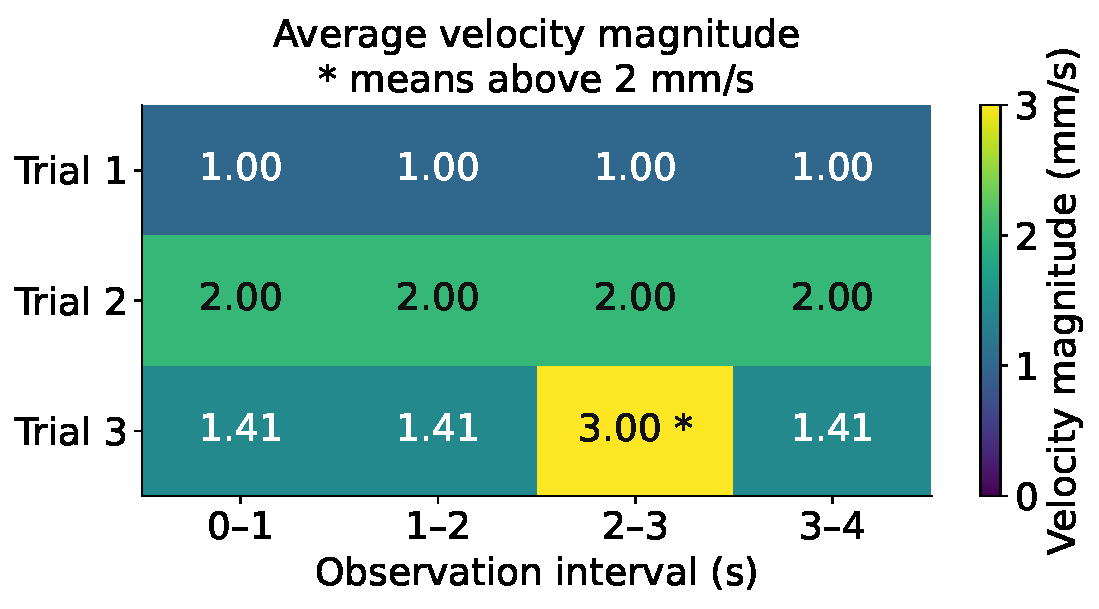
\includegraphics[width=.98\linewidth,height=.69\textheight,keepaspectratio]{speed-shape-map.pdf}\end{frame}
\renewcommand{\notestarget}{notes.pdf\#note-orthogonality-and-length-preservation}
\begin{frame}[t,fragile,label=slide-commutation-with-finite-differences]{Commutation with finite differences}
\[
\frac{Rp_{i+1}-Rp_i}{\Delta t_i}
=R\frac{p_{i+1}-p_i}{\Delta t_i}=Rv_i.
\]
\pause{}
A discrepancy beyond floating-point tolerance suggests an axis or transpose error.
\end{frame}
\renewcommand{\notestarget}{notes.pdf\#note-functions-with-explicit-input-conditions}
\begin{frame}[t,fragile,label=slide-functions-with-explicit-input-conditions]{Functions with explicit input conditions}
Input conditions include
\[
p\in\R^{R\times T\times2},\quad T\geq2,\quad t_{i+1}>t_i.
\]
\pause{}
Check both the input values and the computed velocities for finiteness.
\end{frame}
\renewcommand{\notestarget}{notes.pdf\#note-functions-with-explicit-input-conditions}
\begin{frame}[t,fragile,label=slide-a-geometric-test-suite]{A geometric test suite}
Translation leaves velocity unchanged. Rotation leaves speed unchanged. Rescaling length by $a$ rescales speed by $|a|$.
\pause{}
These relations test the mathematical operation over many arrays without hard-coding every result.
\end{frame}
\end{document}
